% -----------------------------------------------------------------------------
% Lista 01 - Retas e sistemas lineares 2x2
% IDs adotados: L1E01 ... L1E09
% topic={Sistemas 2x2}; dificuldade estimada (1=fácil,2=médio)
% -----------------------------------------------------------------------------

\newcommand{\R}{\mathbb{R}}

\begin{problem}
Determine a solução de cada um dos sistemas lineares
$$\text{(a)}\ \left\{ \begin{array}{rrrrr}
 3x & + &  4y &   = & -8 \\
 9x & + & 10y &   = & -2 \end{array} \right. \ \ \ \ \ \ \ \ \ \ \ \ \ \ \ \\
	\text{(b)}\ \left\{ \begin{array}{rrrrr}
-6x & + &  3y &   = & -4 \\
10x & - &  6y &   = &  5 \end{array} \right.$$
\end{problem}
\begin{solution}
\begin{enumerate}
\item[(a)] Isolando $x$ na primeira equação obtemos $x = \dfrac{-8-4y}{3}$. Substituindo na segunda equação obtemos
$$9 \left( \dfrac{-8-4y}{3}\right) + 10y = -2$$
Multiplicando essa equação por $3$ e simplificando obtemos $-72-6y=-6$ cuja solução é $y=-11$. Substituindo na primeira equação do sistema obtemos $3x-44=-8$ cuja solução é $x=12$. Portanto a solução do sistema é $x=12$ e $y=-11$.
\item[(b)] Isolando $x$ na primeira equação obtemos $x = \dfrac{3y+4}{6}$. Substituindo na segunda equação obtemos
$$10 \left( \dfrac{3y+4}{6}\right) - 6y = 5$$
Multiplicando por $6$ e simplificando obtemos $-6y+40=30$ cuja solução é $y=\dfrac{5}{3}$.
Substituindo na primeira equação do sistema obtemos $-6x+5=-4$ cuja solução é $x=\dfrac{3}{2}$.
Portanto a solução do sistema é $x=\dfrac{3}{2}$ e $y=\dfrac{5}{3}$.
\end{enumerate}
\end{solution}


\begin{problem}
Determine a solução de cada um dos sistemas lineares
$$\text{(a)}\ \left\{ \begin{array}{rrrrr}
 5x & + &  2y &   = & 14 \\
 3x & + &  7y &   = & -9 \end{array} \right. \ \ \ \ \ \ \ \ \ \ \ \ \ \ \ \\
	\text{(b)}\ \left\{ \begin{array}{rrrrr}
 3x & + &  10y &   = & 18 \\
-4x & + &  18y &   = & 23 \end{array} \right.$$ 
\end{problem}
\begin{solution}
\begin{enumerate}
\item[(a)] Multiplicando a primeira equação por 3 e multiplicando a segunda equação por $-5$ obtemos
$$\left\{ \begin{array}{rrrrr}
 15x & + &  6y &   = &  42 \\
-15x & - & 35y &   = &  45 \end{array} \right.$$
Somando estas duas equações obtemos $-29y = 87$ cuja solução é $y=-3$.
Substituindo na primeira equação do sistema linear dado obtemos $5x - 6 = 14$, cuja solução é $x=4$.
Portanto a solução do sistema é $x=4$ e $y=-3$.

\item[(b)] Multiplicando a primeira equação por 4 e multiplicando a segunda equação por $3$ obtemos
$$\left\{ \begin{array}{rrrrr}
 12x & + &  40y &   = & 72 \\
-12x & + &  54y &   = & 69 \end{array} \right.$$
Somando estas duas equações obtemos $94y=141$ cuja solução é $y=\dfrac{3}{2}$.
Substituindo na primeira equação do sistema linear dado obtemos $3x + 15 = 18$ cuja solução é $x=1$.
Portanto a solução do sistema é $x=1$ e $y=\dfrac{3}{2}$.


\end{enumerate}
\end{solution}


\begin{problem}
Em um plano cartesiano represente os pontos $A=(-50,30)$ e $B=(43,-26)$.
A reta $AB$ que liga esses pontos passa pelo primeiro ou pelo terceiro quadrante?
\end{problem}
\begin{solution}
A reta que passa pelos pontos $A$ e $B$ tem equação 
$$y = -\dfrac{56}{93}x - \dfrac{10}{93}$$
Portanto a reta $AB$ intersecta o eixo vertical em $y=-\dfrac{10}{93}$.
Como esse número é negativo e como a reta tem inclinação negativa, concluímos que a reta passa pelo segundo, pelo terceiro e pelo quarto quadrante. A reta não passa pelo primeiro quadrante. A figura a seguir está em escala. Ela ilustra a situação descrita nesta questão.

\centerline{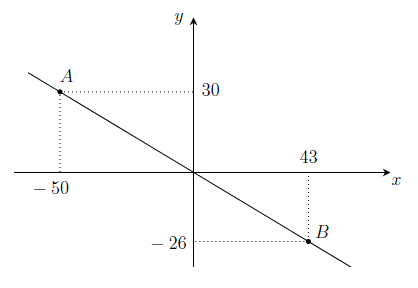
\includegraphics[scale=0.8]{img/sistema2x2_fig8a.png}}

Observe que, como a reta corta os eixos coordenados em pontos próximos da origem, nesta figura não conseguimos identificar se a reta passa pelo primeiro ou pelo terceiro quadrante.
A figura a seguir, fora de escala, evidencia o fato da reta passar pelo segundo, pelo terceiro e pelo quarto quadrante.

\centerline{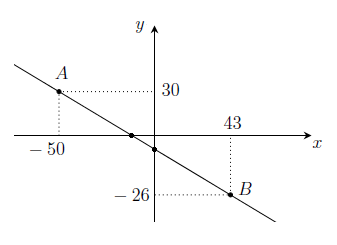
\includegraphics[scale=0.8]{img/sistema2x2_fig8b.png}}
\end{solution}


\begin{problem}
Se $r$ é a reta que passa pelos pontos $A=(13,5)$ e $B=(17,6)$ e se $s$ é a reta que passa pelos pontos $P=(4,6)$ e $Q=(7,-3)$,
determine equações da forma $y=ax+b$ dessas duas retas, faça um esboço dessas retas em um mesmo plano cartesiano e determine as coordenadas do ponto de interseção de $r$ e $s$.
\end{problem}
\begin{solution}
A reta $r$ tem equação $y=x/4+7/4$. A reta $s$ tem equação $y=-3x+18$.
Agora, para determinar o ponto de interseção das retas $r$ e $s$, basta resolver o seguinte sistema linear.
$$\left\{ \begin{array}{rrrrr}
y & = & \dfrac{x}{4}  & +  & \dfrac{7}{4}  \\[12pt]
y & = & -3x           & +  &  18           \end{array} \right.$$
Resolvendo esse sistema obtemos $x=5$ e $y=3$. Portanto as coordenadas do ponto de interseção de $r$ e $s$ são $(5,3)$.

\centerline{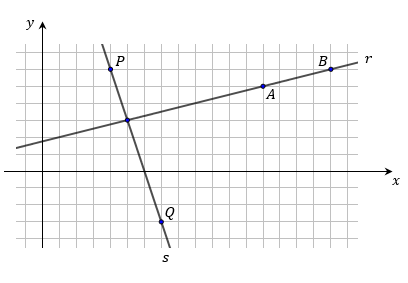
\includegraphics[scale=0.8]{img/sistema2x2_fig6.png}}
\end{solution}


\begin{problem}
Pedro resolveu corretamente o sistema linear a seguir e encontrou como solução $x=-3$ e $y=2$. Em seguida, ele representou corretamente o sistema linear desenhando em um plano cartesiano duas retas. Qual das figuras a seguir pode corresponder ao desenho de Pedro?
$$\left\{ \begin{array}{rrrrr}
	x & + &  3y &   = &  3 \\
-2x & + &   y &   = &  8 \end{array} \right.$$

\medskip
\centerline{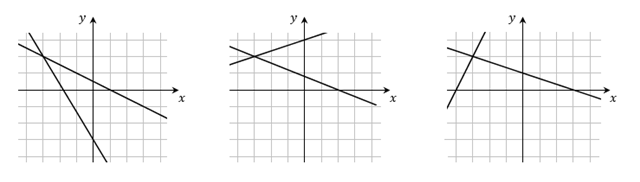
\includegraphics[scale=0.8]{img/sistema2x2_fig4.png}}
\end{problem}
\begin{solution}
Nos três desenhos as retas passam pelo ponto $P=(-3,2)$ que representa a solução do sistema. 
A primeira reta do sistema linear dado intersecta os eixos coordenados em $x=3$ e $y=1$. A segunda reta do sistema linear dado intersecta os eixos coordenados em $x=-4$ e $y=8$. O único desenho que tem essas características é o terceiro desenho.
\end{solution}


\begin{problem}
Seja $r$ a reta que passa pelos pontos $A=(5,4)$ e $B=(14,3)$ e seja $s$ a reta que passa pelos pontos $C=(-6,3)$ e $D=(4,2)$.
Faça um esboço dessas retas em um mesmo plano cartesiano. Após fazer esse desenho é possível saber se as retas $r$ e $s$ são paralelas ou concorrentes? Se elas forem concorrentes, em qual dos quadrantes está o ponto de interseção? 
\end{problem}
\begin{solution}
A reta que passa pelos pontos $A$ e $B$ tem equação $x+9y=41$. A reta que passa pelos pontos $C$ e $D$ tem equação $x+10y=24$.
Resolvendo o sistema linear formado por essas duas equações obtemos como solução $x=194$ e $y=-17$.
Portanto as retas $r$ e $s$ são concorrentes em um ponto do 4$^o$ quadrante.

\centerline{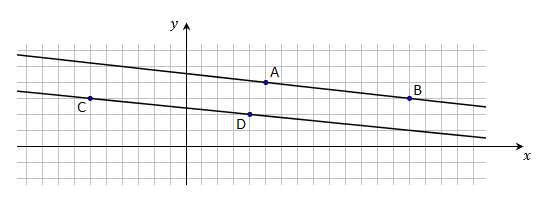
\includegraphics[scale=0.8]{img/sistema2x2_fig7.png}}
\end{solution}


\begin{problem}
Considere o seguinte sistema linear
$$\left\{ \begin{array}{rrrrr}
 -x & + &  7y &   = &  21 \\
 -x & + &  6y &   = & -12 \end{array} \right.$$
André representou corretamente as duas retas desse sistema como na figura a seguir. Como ele não identificou um ponto de interseção entre as retas, concluiu que o sistema é impossível. A conclusão de André está correta?

\medskip
\centerline{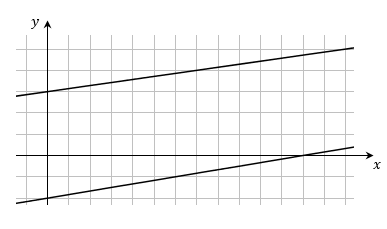
\includegraphics[scale=0.8]{img/sistema2x2_fig5.png}}
\end{problem}
\begin{solution}
Resolvendo o sistema linear dado encontramos a solução $x=210$ e $y=33$.
Portanto as retas não são paralelas e elas tem sim um ponto de interseção. O sistema é possível determinado e a conclusão de André não está correta.
\end{solution}


\begin{problem}
Associe cada sistema linear dado a sua correspondente representação geométrica no plano cartesiano.
$$\text{(A)}\left\{\begin{array}{ccr}
x-2y & = & -4 \\
x+3y & = &  3  \end{array}\right. \ \ \ \\
	\text{(B)}\left\{\begin{array}{ccr}x+2y & = &  4 \\
3x-y & = & -3   \end{array}\right. \ \ \ \\
	\text{(C)}\left\{\begin{array}{ccr}2x+y & = &  4 \\
x-3y & = & -3   \end{array}\right. \ \ \ \\
	\text{(D)}\left\{\begin{array}{ccr}x+2y & = & -4 \\
3x+y & = &  3   \end{array}\right.$$

\medskip
\centerline{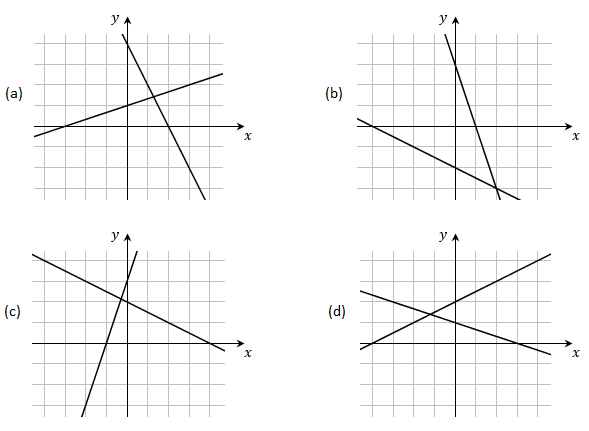
\includegraphics[scale=0.8]{img/sistema2x2_fig3.png}}
\end{problem}
\begin{solution}
Para cada sistema linear dado, represente as restas em um plano cartesiano. 
Você pode fazer isso em uma folha de papel ou no GeoGebra. 
Após fazer as figuras corretas, a correspondência é (A)-(d), (B)-(c), (C)-(a) e (D)-(b).
\end{solution}


\begin{problem}
Considere o seguinte sistema nas variáveis $x$ e $y$.
$$\left\{ \begin{array}{rrrrr}
3x & + &  ay &  = &   1 \\
ax & + & 12y &  = &  -2 \end{array} \right.$$
Determine condições sobre o coeficiente $a$ para que esse sistema seja possível e determinado (uma única solução), seja impossível (nenhuma solução) e seja possível e indeterminado (infinitas soluções).
\end{problem}
\begin{solution}
Isolando $x$ na primeira equação obtemos $x=\dfrac{1-ay}{3}$. Substituindo na segunda equação obtemos
$$a \left( \dfrac{1-ay}{3} \right) + 12y = -2$$
Multiplicando por 3 e simplificando obtemos
$$(36-a^2)y = -6-a$$
Para calcular o valor de $y$ é necessário que $36-a^2$ seja diferente de zero. Se esse é o caso, obtemos
$$y = \dfrac{-6-a}{36-a^2} = \dfrac{-6-a}{(6+a)(6-a)} = -\dfrac{1}{6-a} = \dfrac{1}{a-6}$$
Substituindo na expressão de $x$ obtemos 
$$x = \dfrac{1-ay}{3}  = \dfrac{1 - a \, \dfrac{1}{a-6} }{3} = \dfrac{2}{6-a}$$
Logo se $a^2-36 \neq 0$, então o sistema tem uma única solução dada por
$$x = \dfrac{2}{6-a} \ \ \ \ \text{e} \ \ \ \ y = \dfrac{1}{a-6}$$
Como $a^2-36=0$ somente se $a=6$ ou se $a=-6$, concluímos que se $a \neq 6$ ou se $a \neq-6$ então o sistema admite uma única solução.
Vamos  analisar os casos $a=6$ e $a=-6$ separadamente.

\medskip

\begin{itemize}
\item Substituindo $a=6$ no sistema linear dado obtemos
$$\left\{ \begin{array}{rrrrr}
3x & + &  6y &  = &   1 \\
6x & + & 12y &  = &  -2 \end{array} \right.$$
Dividindo a segunda equação por 2 obtemos o sistema linear
$$\left\{ \begin{array}{rrrrr}
3x & + &  6y &  = &   1 \\
3x & + &  6y &  = &  -1 \end{array} \right.$$
Como estas duas equações são contraditórias, concluímos que para $a=6$ o sistema é impossível.


\item Substituindo $a=-6$ no sistema linear dado obtemos
$$\left\{ \begin{array}{rrrrr}
 3x & - &  6y &  = &   1 \\
-6x & + & 12y &  = &  -2 \end{array} \right.$$
Nesse caso, se multiplicarmos a primeira equação por $-2$ obtemos a segunda equação. Isso implica que as retas dadas por essas duas equações são coincidentes e que qualquer ponto sobre essa reta comum é uma solução do sistema. Portanto para $a=-6$ o sistema é possível e determinado.
\end{itemize}

\medskip
Observação. Para uma interpretação geométrica, em um arquivo GeoGebra, crie um controle deslizante $a$
percorrendo o intervalo de $-10$ até $10$  e crie as retas de equações $3x+ay=1$ e $ax+12y=-2$. Variando $a$, observe que quase sempre essas retas são concorrentes em um único ponto. Quando $a=6$ as retas ficam paralelas e quanto $a=-6$ as retas ficam coincidentes. Habilitando o rastro do ponto $P$ de interseção dessas retas, veja que $P$ varia sobre uma reta quando $a\in\R$.
Como desafio, determine a equação dessa reta. A resposta é: $P$ varia sobre a reta de equação $y=-\dfrac{x}{2}$.
\end{solution}


